\section{FUNCIONALIDADES DO MFIT\label{introducao}}

\hspace*{1.25cm}Neste cap�tulo ser� explicado todas as funcionalidades do MFIT.

\subsection{Carregar um V�deo\label{carrega_video}}

Nesta se��o detalharemos os passos necess�rios para se carregar um V�deo.

\begin{enumerate}

\item{Abra o MFIT (Figura \ref{img:mfit_aberto})}

\begin{figure}[h|top]
 \centering
 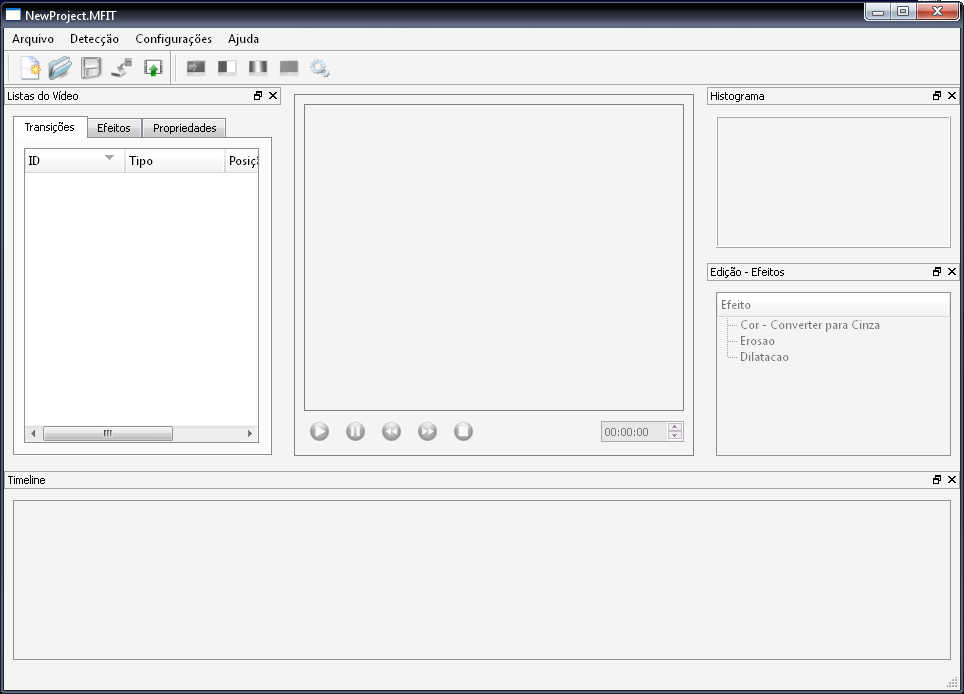
\includegraphics[width=0.5\linewidth]{imagens/mfit_aberto.png}
 \caption{MFIT Aberto sem V�deo carregado.}
 Fonte: Autor.
 \label{img:mfit_aberto}
\end{figure}

\item{Clique com o bot�o direito no menu "Arquivo", op��o "Carregar V�deo".
Se preferir, pressione as teclas Ctrl+Shif+O (Figura \ref{img:carregar2}). }

\begin{figure}[h|top]
 \centering
 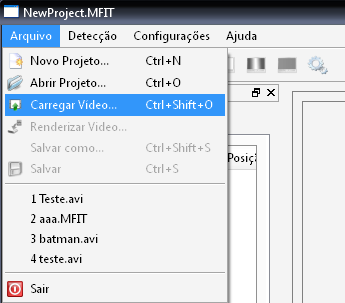
\includegraphics[width=0.5\linewidth]{imagens/carregar2.png}
 \caption{Menu "Arquivo", op��o "Carregar V�deo" .}
 Fonte: Autor.
 \label{img:carregar2}
\end{figure}

\item{Na janela que abrir�, selecione um V�deo v�lido (com extens�o .AVI) e de um duplo clique (Figura \ref{img:carregar3}). }

\begin{figure}[h|top]
 \centering
 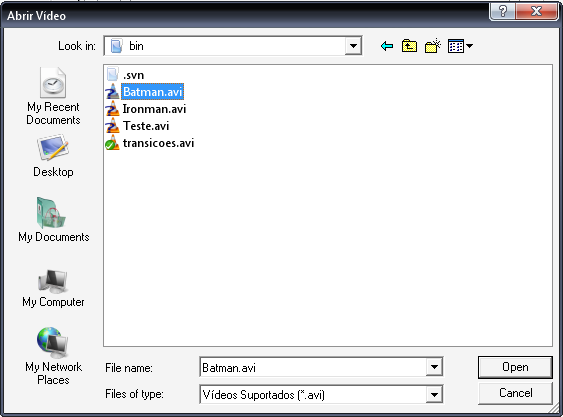
\includegraphics[width=0.5\linewidth]{imagens/carregar3.png}
 \caption{Selecionando um V�deo v�lido.}
 Fonte: Autor.
 \label{img:carregar3}
\end{figure}

\item{Ap�s alguns instantes o v�deo estar� aberto, e sua timeline estar� montada.
Note que uma janela se abrir�, questionando se o processo de detec��o de transi��es deve ser iniciado.
Por hora, clique em cancelar (Figura \ref{img:carregar4}). }

\begin{figure}[h|top]
 \centering
 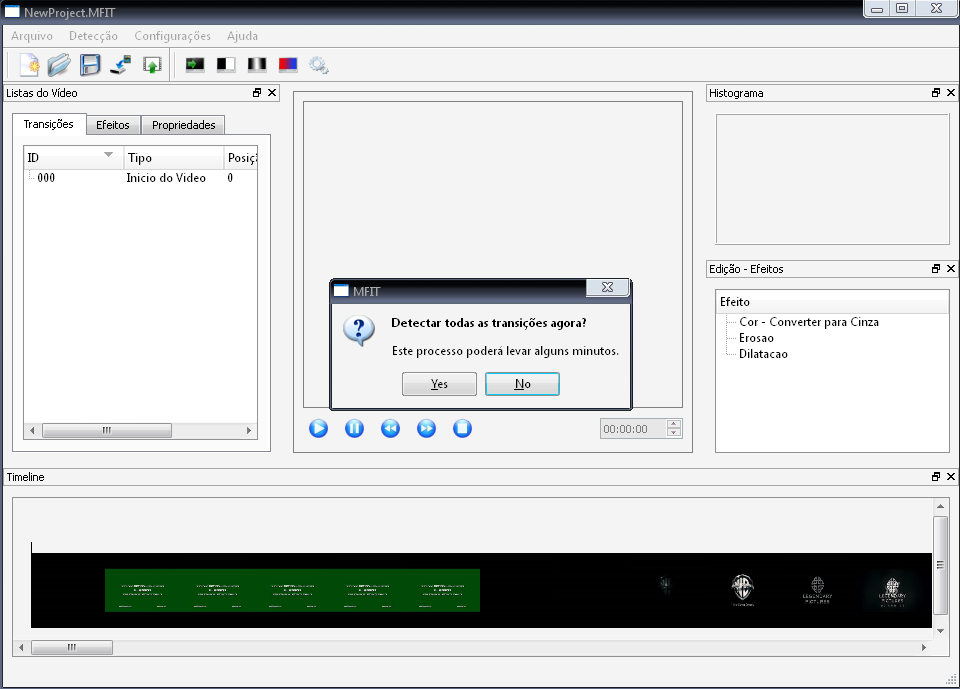
\includegraphics[width=0.5\linewidth]{imagens/carregar4.png}
 \caption{V�deo carregado e janela questionando o processo de detec��o.}
 Fonte: Autor.
 \label{img:carregar4}
\end{figure}

\item{Processo finalizado, o V�deo est� pronto para se efetuar todas as opera��es poss�veis (Figura \ref{img:carregar5}). }

\begin{figure}[h|top]
 \centering
 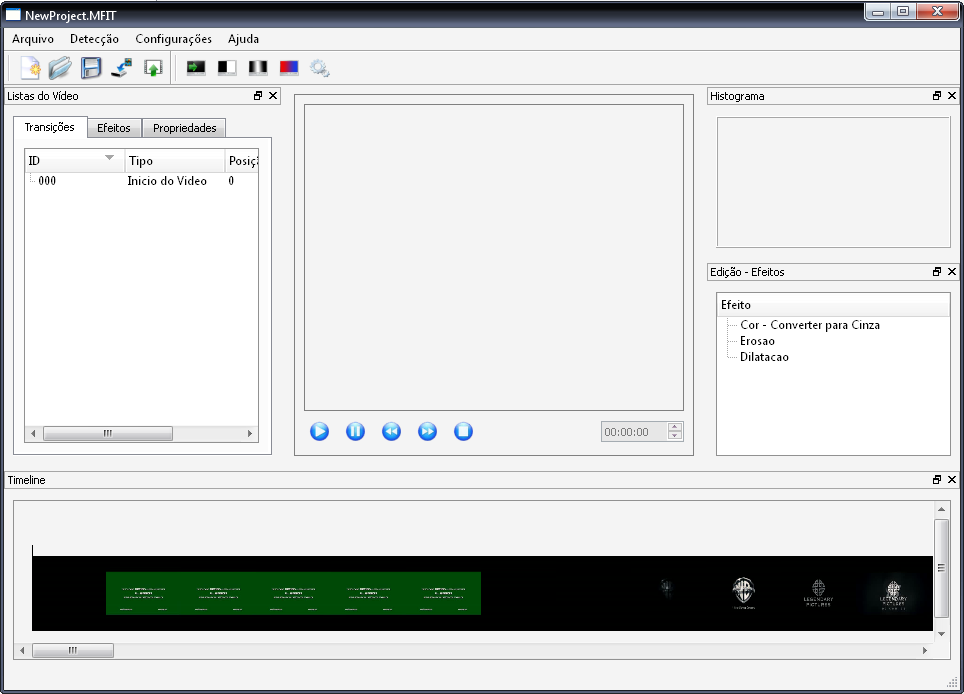
\includegraphics[width=0.5\linewidth]{imagens/carregar5.png}
 \caption{Fim do processo.}
 Fonte: Autor.
 \label{img:carregar5}
\end{figure}

\end{enumerate}
